\chapter{USB}\label{cap:usb}

El \emph{Universal Serial Bus}(USB\footnote{V\'ease - http://www.usb.org}) es
un bus serial est\'andar que hace de interfaz entre un dispositivo y una
computadora.
Dicha estandarizaci\'on es llevada acabo por el \emph{F\'orum de
Implementadores de USB} (USB Implementers Forum, USB-IF\footnote{V\'ease -
http://www.usb.org/about}). 
Actualmente el est\'andar se encuentra en su versi\'on 3.0\footnote{V\'ease -
http://www.usb.org/developers/docs/}, aunque la mayor\'ia de las
implementaciones comerciales solo soportan el ent\'andar \emph{2.0}.

%%%%%%%%%%%%%%%%%%%%%%%%%%%%%%%%%%%%%%%%%%%%%%%%%%%%%%%%%%%%%%%%%%%%%%%%%%%%%%
%%%%%%%%%%%%%%%%%%%%%%%%%%%%%%%%%%%%%%%%%%%%%%%%%%%%%%%%%%%%%%%%%%%%%%%%%%%%%%
%\clearpage
%\section{Historia}
%No me gusta como titulo 'historia' habria que pensar otra cosa

%%%%%%%%%%%%%%%%%%%%%%%%%%%%%%%%%%%%%%%%%%%%%%%%%%%%%%%%%%%%%%%%%%%%%%%%%%%%%%
%%%%%%%%%%%%%%%%%%%%%%%%%%%%%%%%%%%%%%%%%%%%%%%%%%%%%%%%%%%%%%%%%%%%%%%%%%%%%%
\clearpage
\section{Decripci\'on}
% Aca iria el funcionamiento del USB, diferenciado por \subsection{}
% Por ahora me estoy basando en la spec 2.0 oficial.
La especificaci\'on USB provee una serie de atributos con los cuales se pueden
implementar dispositivos seg\'un el precio/rendimiento deseado.

%%%%%%%%%%%%%%%%%%%%%%%%%%%%%%%%%%%%%%%%%%%%%%%%%%%%%%%%%%%%%%%%%%%%%%%%%%%%%%
\subsection{Caracter\'isticas}
Del amplio rango de caracter\'isticas definidas en el est\'andar, es posible
agruparlas en ocho categor\'ias:
% Reescribir lo de arriba y agregar mas

\begin{itemize}
 \item Facilidad de uso para el usuario final
 \item Amplio rango de aplicaciones
 \item Ancho de banda is\'ocrono
 \item Flexibilidad
 \item Robustez
 \item Sinergia con la industria de la PC
 \item Implementaci\'on de bajo costo
 \item De arquitectura actualizable
\end{itemize}

La combinaci\'on de estas caracter\'isticas hacen a la versatilidad del
ent\'andar, ya que permiten implementar todo tipo de dispositivos seg\'un la
carga, versatilidad, eficiencia, precio, velocidad y dem\'as atributos que
puedan inferir en un diese\~no.\\

Para la veri\'on 2.0 de la epecificaci\'on, el protocolo soporta tres
velocidades de transmisi\'on como se muestra en la
tabla \ref{tab:velocidad_usb}.

\begin{table}[ht]
\centering
% use packages: array,booktabs
\begin{tabular}{|c|c|}        \hline
High Speed & 480 Mbits/seg \\ \hline 
Full Speed & 12 Mbits/seg  \\ \hline
Low Speed & 1.5 Mbits/seg  \\ \hline
\end{tabular}
\caption{Velocidades de USB} 
\label{tab:velocidad_usb}
\end{table}

%%%%%%%%%%%%%%%%%%%%%%%%%%%%%%%%%%%%%%%%%%%%%%%%%%%%%%%%%%%%%%%%%%%%%%%%%%%%%%
\subsection{Arquitectura}

USB es un \emph{bus} cableado que soporta conexiones entre un \emph{host} y
gran rango de perif\'ericos. Dicho \emph{bus} permite la conexi\'on,
configuraci\'on, uso y desconexi\'on de un dispositivo mientras el \emph{host}
y dem\'as perif\'ericos est\'an en funcionamiento. \\

Un sistema USB se  define seg\'un tres grandes \'areas:

\begin{itemize}
 \item Interconexi\'on USB
 \item Dispositivo USB
 \item \emph{Host} USB
\end{itemize}

%%%%%%%%%%%%%%%%%%%%%%%%%%%%%%%%%%%%%%%%%%%%%%%%%%%%%%%%%%%%%%%%%%%%%%%%%%%%%%
\subsubsection{Caracter\'isticas el\'ectricas}

USB usa cuatro cables para alimentaci\'on y se\~nal. La se\~nal viaja a
trav\'es
de un par trenzado diferencial y se encuentra codificada con Non Return to Zero
Inverted (NRZI). En la figura \ref{fig:electric_usb} se muestra un diagrama de
un cable
USB.

\begin{figure}[htp]
\centering
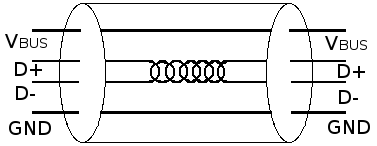
\includegraphics[scale=0.5]{./img/electric_usb.png}
\caption{Cable USB.}
\label{fig:electric_usb}
\end{figure}

Al ser un par diferencial, el host interpreta un \emph{1} diferencial cuando D+
es 200 mV mayor que D- y un \emph{0} diferencial cuando D- es 200 mV mayor que
D+. 
Los dispositivos USB indican su velocidad mediante una resistencia de
\emph{pull-up} a 3.3 V. En el caso de un \emph{full speed device} se col\'oca
una resistencia de 1.5K en D+ a 3.3 V, y para \emph{low speed device} se coloca
una resistencia de 1.5K a 3.3 V, como se muestra en la figura
\ref{fig:electric_speed_usb}.
Algunos fabricantes sulen integrar estas resistencias de \emph{pull-up} dentro
de sus \emph{chips} para ser activadas mediante software.

\begin{figure}[htp]
\centering
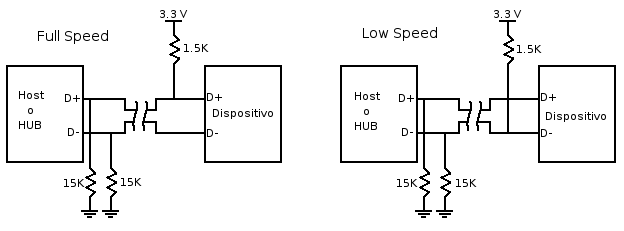
\includegraphics[scale=0.5]{./img/electric_speed_usb.png}
\caption{Velocidad USB.}
\label{fig:electric_speed_usb}
\end{figure}


%%%%%%%%%%%%%%%%%%%%%%%%%%%%%%%%%%%%%%%%%%%%%%%%%%%%%%%%%%%%%%%%%%%%%%%%%%%%%%
\subsection{Interconexi\'on USB}

La interconexi\'on USB define la manera en la que los dispositivos USB se
conectan entre si y con el \emph{host}. 

%%%%%%%%%%%%%%%%%%%%%%%%%%%%%%%%%%%%%%%%%%%%%%%%%%%%%%%%%%%%%%%%%%%%%%%%%%%%%%
\subsubsection{Topolog\'ia del bus}

USB usa una topolog\'ia de estrella por niveles. Un \emph{hub}\footnote{La
palabra \emph{hub} se traduce al castellano como \emph{centro}, pero su
traducci\'on no sera usada en este documento por cuestiones pr\'acticas.}
est\'a ubicado al centro de cada estrella. Las conexiones cableadas se dan
entre el \emph{host} y un \emph{hub} o funci\'on, entre \emph{hub} y
\emph{hub}, o entre un \emph{hub} y una funci\'on. \\

Debido a cuestiones de latencia, el n\'umero m\'aximo de niveles permitido es
siete, incluida la ra\'iz. La figura \ref{fig:usb_topology} muestra un esquema
de la topolog\'ia.

\begin{figure}[htp]
\centering
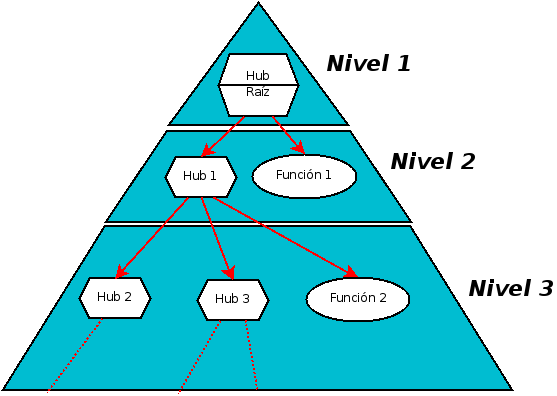
\includegraphics[scale=0.5]{./img/usb_topology.png}
\caption{Topolog\'ia del bus USB.}
\label{fig:usb_topology}
\end{figure}


%%%%%%%%%%%%%%%%%%%%%%%%%%%%%%%%%%%%%%%%%%%%%%%%%%%%%%%%%%%%%%%%%%%%%%%%%%%%%%
\subsection{\emph{Host} USB}

La especificaci\'on admite un solo \emph{Host} para un todo sistema USB. La
interf\'az USB del \emph{host}, se la denomina \emph{Host
Controller}\footnote{Al igual que con \emph{host}, esta palabra se mantedr\'a
en ingles.}. La implementaci\'on de un \emph{Host Controller} puede ser una
combinaci\'on de hardware, firmware o software. El \emph{hub} ra\'iz esta
integrado en el sistema \emph{host}, proveyendo puntos de acceso.
En la versi\'on 1.1 de la especificaci\'on, exist\'ian dos tipo de
controladores de \emph{hots}; \emph{Universal Host Controller Interface}
(UHCI)\footnote{Desarrollada por Intel} y \emph{Open Host Controller Interface}
(OHCI)\footnote{Desarrollada por Compaq, Microsoft y National Semiconductors}.
Luego con para le versi\'on 2.0 de la especificaci\'on de defini\'o un tercer
controlador; \emph{Enhanced Host Controller Interface} (EHCI)\footnote{Que
luego pasar\'ia a convertirse en el est\'andar mas usado.}


%%%%%%%%%%%%%%%%%%%%%%%%%%%%%%%%%%%%%%%%%%%%%%%%%%%%%%%%%%%%%%%%%%%%%%%%%%%%%%
\subsection{Dispositivo USB}

Los dispositivos USB pueden ser dispositivos funcionales o bien \emph{hubs}.
En ambos casos deben ser capaces de entender el protocolo USB y responder a
peticiones est\'andares USB adem\'as de cumplir su funci\'on intr\'inseca. 

% Explicar --- UHCI, OHCI, EHCI
%\begin{Huge} TERMINAR!!! \end{Huge}


El protocolo USB define capas de abstracci\'on, cada cual con una funcionalidad
espec\'ifica. Normalmente los \emph{chips} manejan las capas mas bajas, para
abstraer al usuario de todo lo que ocurre en lo mas bajo del protocolo.\\

Una transacci\'on USB consiste de los siguientes paquetes:
\begin{itemize}
 \item Token (paquete cabecera)
 \item Data (opcional)
 \item Status (handshaking)
\end{itemize}

Los paquetes USB tienen ciertos campos comunes: 
\begin{itemize}
 \item Sync: Es un campo de sincronismo y todos los paquetes deben comenzar
con uno.
 \item PID: Es el identificador de paquete que informa el tipo de paquete que
es.
 \item ADDR: Es la direcci\'on a la cual esta asignado el paquete
 \item ENDP: Este campo de 4 bits permite direccionar hasta 16
\emph{endpoints}.
 \item CRC: Lleva la informaci\'on de un chequeo de redundancia c\'iclica de
los datos
 \item EOP: Este campo indica la finalizaci\'on del paquete.
\end{itemize}

%%%%%%%%%%%%%%%%%%%%%%%%%%%%%%%%%%%%%%%%%%%%%%%%%%%%%%%%%%%%%%%%%%%%%%%%%%%%%%
\subsubsection{Paquete \emph{Token}}
Los paquetes \emph{token} son usados para indicar el tipo de transacci\'on que
se realizar\'a. Existen tres tipos de paquetes \emph{token}:

\begin{itemize}
 \item IN - Informa al dispositivo USB que el host desea leer informaci\'on
 \item OUT - Informa al dispositivo USB que el host desea escribir
informaci\'on
 \item Setup - Es usado para comenzar transferencias de control
\end{itemize}

Un paquete \emph{token} esta formado por los siguientes campos mostrados en la
tabla \ref{tab:usb_token_fields}


\begin{table}[ht]
\centering
% use packages: array,booktabs
\begin{tabular}{|c|c|c|c|c|c|} \hline
Sync & PID & ADDR & ENDP & CRC5 & EOP\\ \hline
\end{tabular}
\caption{Campos Token} 
\label{tab:usb_token_fields}
\end{table}


%%%%%%%%%%%%%%%%%%%%%%%%%%%%%%%%%%%%%%%%%%%%%%%%%%%%%%%%%%%%%%%%%%%%%%%%%%%%%%
\subsubsection{Paquete \emph{Data}}
Un paquete \emph{data} esta formado por los siguientes campos mostrados en la
tabla \ref{tab:usb_data_fields}

\begin{table}[ht]
\centering
% use packages: array,booktabs
\begin{tabular}{|c|c|c|c|c|} \hline
Sync & PID & DATA & CRC16 & EOP\\ \hline
\end{tabular}
\caption{Campos Data} 
\label{tab:usb_data_fields}
\end{table}


%%%%%%%%%%%%%%%%%%%%%%%%%%%%%%%%%%%%%%%%%%%%%%%%%%%%%%%%%%%%%%%%%%%%%%%%%%%%%%
\subsubsection{Paquete \emph{Status}}
Los paquetes \emph{status} son usados para indicar el tipo de estado de la
transacci\'on. Existen tres tipos de paquetes \emph{status}:

\begin{itemize}
 \item ACK - Reconocimiento de que el paquete fue recibido.
 \item NAK - Avisa de que el dispositivo no puede recibir ni enviar datos.
 \item STALL - Significa que el dispositivo necesita la intervenci\'on del
host.
\end{itemize}

Un paquete \emph{status} esta formado por los siguientes campos mostrados en la
tabla \ref{tab:usb_status_fields}.

\begin{table}[ht]
\centering
% use packages: array,booktabs
\begin{tabular}{|c|c|c|} \hline
Sync & PID & EOP\\ \hline
\end{tabular}
\caption{Campos Status} 
\label{tab:usb_status_fields}
\end{table}


%%%%%%%%%%%%%%%%%%%%%%%%%%%%%%%%%%%%%%%%%%%%%%%%%%%%%%%%%%%%%%%%%%%%%%%%%%%%%%
%%%%%%%%%%%%%%%%%%%%%%%%%%%%%%%%%%%%%%%%%%%%%%%%%%%%%%%%%%%%%%%%%%%%%%%%%%%%%%
\clearpage
\section{Enpoints}\label{cap:usb_endpoints}
Un aspecto muy importante del est\'andar USB es la forma en la que se logra la
comunicaci\'on entre el host y el dispositivo.
Un \emph{endpoint} es un buffer \'unico que define la punta extrema de un
canal de comunicaci\'on. La identificaci\'on de un endpoint en particular se
lleva a cabo mediante un campo de 4 bits permitiendo un m\'aximo de 16
endpoints. Cada enpoint funciona como emisor o receptor de datos como se ve en
la figura \ref{fig:usb_endpoints}.

\begin{figure}[htp]
\centering
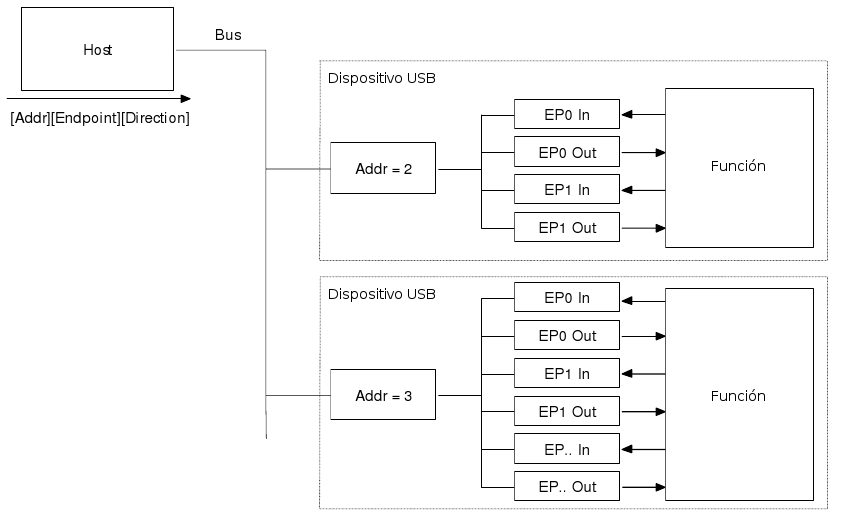
\includegraphics[scale=0.5]{./img/usb_endpoints.png}
\caption{Endpoints de USB.}
\label{fig:usb_endpoints}
\end{figure}

Entonces si por ejemplo el host emite un pedido de descripci\'on de dispositivo
(\emph{device descriptor request}) el dispositivo va a determinar por medio de
el campo \emph{ADDR} si el pedido esta dirigido hacia \'el, y luego copiar\'a
el dato en el endpoint correspondiente al que indica el campo \emph{ENDP}, que
luego podr\'a ser le\'ido por la aplicaci\'on embebida en el dispositivo.\\

El enpoint 0 debe existir en todos los dispositivos, ya cumple la funci\'on
espec\'ifica de realizar el handshaking y todo el control en una
comunicaci\'on USB. 


%%%%%%%%%%%%%%%%%%%%%%%%%%%%%%%%%%%%%%%%%%%%%%%%%%%%%%%%%%%%%%%%%%%%%%%%%%%%%%
%%%%%%%%%%%%%%%%%%%%%%%%%%%%%%%%%%%%%%%%%%%%%%%%%%%%%%%%%%%%%%%%%%%%%%%%%%%%%%
\clearpage
\section{Transferencias USB}
La especificaci\'on USB define cuatro tipos de transferencia:

\begin{itemize}
 \item Control
 \item Interrupt
 \item Isochronous 
 \item Bulk
\end{itemize}

Debido a el alcance de \'este trabajo solo se desarrollar\'an las
transferencias \emph{Control} y \emph{Bulk}, que fueron las usadas durante el
desarrollo del proyecto.


%%%%%%%%%%%%%%%%%%%%%%%%%%%%%%%%%%%%%%%%%%%%%%%%%%%%%%%%%%%%%%%%%%%%%%%%%%%%%%
\subsection{Control}
Las transferencias de control son usadas para petici\'on y reporte de estados o
emisi\'on de ordenes. Este tipo de transferencia posee tres etapas distintas:

\begin{itemize}
 \item Setup:
		Durante esta etapa se realiza la petici\'on de datos.
 \item Data:
		En esta etapa se realiza el intercambio de datos y puede consistir de
varias transferencias \emph{IN} o \emph{OUT} seg\'un corresponda. 
 \item Status:
		Esta etapa se realiza al finalizar la transferencia de control y
determina el \'exito o no de la operaci\'on.
\end{itemize}


%%%%%%%%%%%%%%%%%%%%%%%%%%%%%%%%%%%%%%%%%%%%%%%%%%%%%%%%%%%%%%%%%%%%%%%%%%%%%%
\subsection{Bulk}
Las transferencias tipo \emph{bulk}, son usadas para transmisi\'on de grandes
pedazos de datos. \'Este tipo transferencias provee correcci\'on de datos
con un campo \emph{CRC} de 16 bits y un mecanismo de detecci\'on y
re-trasmisi\'on de errores para asegurar la integridad de los mismos.\\

Las transferencias bulk no poseen un ancho de banda asignado, por lo cual no
aseguran latencia alguna.\\

Las transacciones bulk pueden ser de tipo \emph{IN} o \emph{OUT} como se ve en
la figura \ref{fig:usb_bulk_transaction}.

\begin{figure}[htp]
\centering
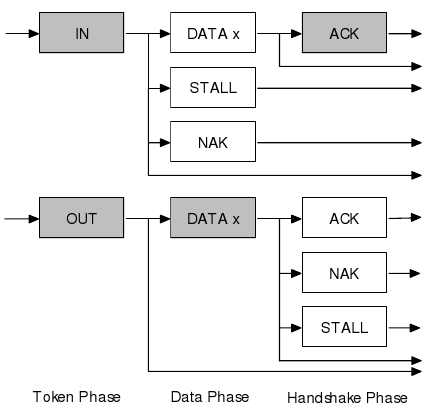
\includegraphics[scale=0.5]{./img/usb_bulk_transaction.png}
\caption{Transacci\'on Bulk.}
\label{fig:usb_bulk_transaction}
\end{figure}


%%%%%%%%%%%%%%%%%%%%%%%%%%%%%%%%%%%%%%%%%%%%%%%%%%%%%%%%%%%%%%%%%%%%%%%%%%%%%%
%%%%%%%%%%%%%%%%%%%%%%%%%%%%%%%%%%%%%%%%%%%%%%%%%%%%%%%%%%%%%%%%%%%%%%%%%%%%%%
\clearpage
\section{Descriptores USB}
% Revisar pagina 240 de la spec usb 2.0 gr\'afico de estados para agregar
% Agregar proceso de enumeraci\'on de la spec pag 243	
Los descriptores USB son estructuras de datos con formatos especif\'icos, en
los cuales se almacena todos los atributos del dispositivo.
Cada descriptor comienza con un campo donde se almacena el tama\~no de dicho
descriptor, seguido inmediatamente por un campo que identifica el tipo de
descriptor.\\
Entre los descriptores mas comunes se encuentran:

\begin{itemize}
 \item Device: Cada dispositivo tiene un solo descriptor \emph{device}, y
\'estos poseen informaci\'on b\'asica sobre \'el. Entre otras cosas este
descriptor tiene un n\'umero identificador del vendedor y el dispositivo en
si. Tiene adem\'as un campo con la informaci\'on de cuantas configuraciones
soporta el dispositivo.

 \item Configuration: Este descriptor posee entre otras cosas el tipo de
alimentaci\'on y el n\'umero de interfaces configuradas del dispositivo.

 \item Interface: Este descriptor puede ser visto como una cabecera con
informaci\'on sobre un grupo de endpoints.

 \item Enpoint: Este descriptor posee toda la informaci\'on necesaria para
caracterizar cada endpoint. Entre otras cosas aqu\'i se define el tipo de
transferencia que usa el endpoint (bulk, interrupt, isochronous, control), el
tama\~no de los paquetes, etc. El endpoint 0 siempre es considerado de control
y debe estar configurado.

 \item String: Estos descriptores poseen informaci\'on legible por humanos que
pueden ser indexados por otros descriptores. 

\end{itemize}

Los descriptores pueden ser ordenados jer\'arquicamente seg\'un se ve en la
figura \ref{fig:usb_descriptors}

\begin{figure}[htp]
\centering
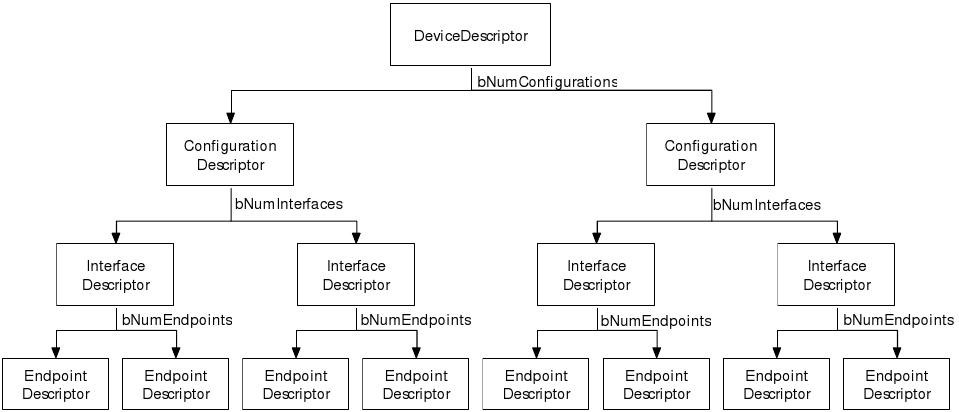
\includegraphics[scale=0.4]{./img/usb_descriptors.png}
\caption{Descriptores USB.}
\label{fig:usb_descriptors}
\end{figure}

%%%%%%%%%%%%%%%%%%%%%%%%%%%%%%%%%%%%%%%%%%%%%%%%%%%%%%%%%%%%%%%%%%%%%%%%%%%%%%
%%%%%%%%%%%%%%%%%%%%%%%%%%%%%%%%%%%%%%%%%%%%%%%%%%%%%%%%%%%%%%%%%%%%%%%%%%%%%%
\clearpage
\section{Estados USB}
Los dispositivos USB poseen varios estados definidos por los cuales pueden
transicionar durante su uso.
El diagrama de estados completo de un dispositivo USB puede verse en la figura
\ref{fig:usb_states}.


% Spec 2,.0 pag 240
\begin{figure}[htp]
\centering
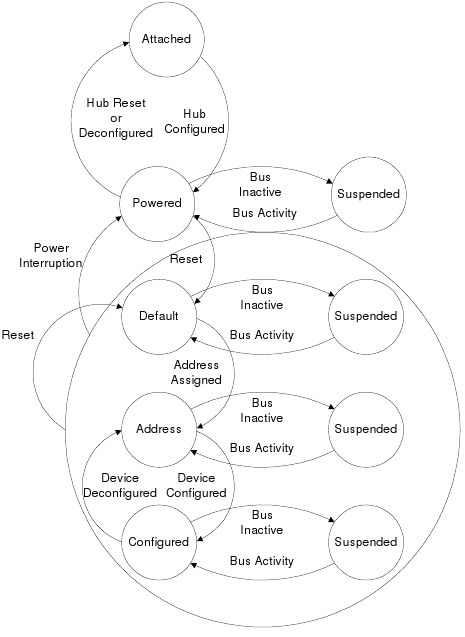
\includegraphics[width=10cm]{./img/usb_states.png}
\caption{Estados USB.}
\label{fig:usb_states}
\end{figure}


En la tabla \ref{tab:usb_states}, se puede apreciar una breve explicaci\'on de
cada estado

% Spec 2,.0 pag 241
\begin{table}[ht]
\begin{scriptsize}
\centering
\begin{tabular*}{\textwidth}{@{\extracolsep{\fill}}|c|c|c|c|c|c|p{5cm}|} \hline

% Header Titles
\rowcolor[gray]{.9}
Attached & Powered & Default & Address & Configured & Suspended
& Descripci\'on\\ \hline

% Table fill
% 1 %
No & -- & -- & -- & -- & -- & 
El dispositivo no est\'a enchufado\\
\hline
% 2 %
Si & No & -- & -- & -- & -- & 
El dispositivo esta enchufado pero no alimentado.\\
\hline 
% 3 %
Si & Si & No & -- & -- & -- &
El dispositivo se encuentra enchufado y alimentado, pero no ha sido
reseteado.\\
\hline
% 4 %
Si & Si & Si & No & -- & -- &
El dispositivo se encuentra enchufado, alimentado y ha sido reseteado, pero no
se le ha asignado una direcci\'on \'unica.\\
\hline
% 5 %
Si & Si & Si & Si & No & -- &
El dispositivo esta enchufado, alimentado, ha sido reseteado y se le ha
asignado una direcci\'on \'unica, pero no ha sigo configurado.\\
\hline
% 6 %
Si & Si & Si & Si & Si & No &
El dispositivo est\'a enchufado, alimentado, ha sido reseteado, se le ha
asignado una direcci\'on \'unica, ha sido configurado y no esta suspendido. El
host puede hacer uso del dispositivo ahora.\\
\hline
% 7 &
Si & Si & -- & -- & -- & Si &
El dispositivo se encuentra como m\'inimo enchufado y alimentado, pero no ha
presentado actividad alguna en los \'ultimos 3 ms, por lo que el dispositivo se
encuentra suspendido y no puede ser usado por el host.\\
\hline 

\end{tabular*}
\caption{Estados USB.} 
\label{tab:usb_states}
\end{scriptsize}
\end{table}

%%%%%%%%%%%%%%%%%%%%%%%%%%%%%%%%%%%%%%%%%%%%%%%%%%%%%%%%%%%%%%%%%%%%%%%%%%%%%%
%%%%%%%%%%%%%%%%%%%%%%%%%%%%%%%%%%%%%%%%%%%%%%%%%%%%%%%%%%%%%%%%%%%%%%%%%%%%%%
\clearpage
\section{Enumeraci\'on del bus USB}
El proceso de enumeraci\'on determina si un dispositivo se ha conectado al
bus, a que puerto, sus configuraciones, interfaces, etc.
A continuaci\'on se listan los acciones que se llevan a cabo durante el
proceso de enumeraci\'on.

% Spec 2.0 pag 243
\begin{enumerate}
 % 1 %
 \item El hub a el cual el dispositivo esta conectado informa al host del
evento. En este paso el dispositivo se encuentra \emph{POWERED} y el puerto al
cual esta enchufado se encuentra deshabilitado.
 % 2 %
 \item El host determina la naturaleza del cambio consult\'andole al hub.
 % 3 %
 \item El host conoce ahora el puerto al cual se ha conectado el dispositivo y
espera 100 ms para que se normalice su alimentaci\'on. El host habilita el
puerto y env\'ia una petici\'on de \emph{reset}.
 % 4 %
 \item El hub ejecuta el pedido de \emph{reset} para ese puerto y luego el
puerto queda habilitado. El dispositivo pasa a el estado \emph{DEFAULT} y no
puede consumir mas de 100 mA. Todos sus registros han sidos reseteados y
responde a la direcci\'on por defecto.
 % 5 %
 \item El host asigna una direcci\'on \'unica al dispositivo y esta pasa al
estado \emph{ADDRESS}.
 % 6 %
 \item El host lee del dispositivo el tama\~no de datos que puede recibir antes
de que \'este reciba la direcci\'on.
 % 7 %
 \item El host lee toda la configuraci\'on de dispositivo.
 % 8 %
 \item Basado en la configuraci\'on obtenida, el host asigna un valor de
configuraci\'on al dispositivo y \'este pasa a el estado de \emph{CONFIGURED}.
Desde el punto de vista del dispositivo \'este se encuentra listo para ser
usado.
\end{enumerate}

%%%%%%%%%%%%%%%%%%%%%%%%%%%%%%%%%%%%%%%%%%%%%%%%%%%%%%%%%%%%%%%%%%%%%%%%%%%%%%
%%%%%%%%%%%%%%%%%%%%%%%%%%%%%%%%%%%%%%%%%%%%%%%%%%%%%%%%%%%%%%%%%%%%%%%%%%%%%%
\newpage
\section{PIC18F4550 USB}
% Habra que ponerle el cosito de copyright al lado de Microchip?
La familia de microcontroladores PIC18FX455/X550 de Microchip provee
conexi\'on USB de tipo \emph{full} y \emph{high-speed}. Dicha comunicaci\'on
se lleva acabo mediante lo que Microchip denomina \emph{USB Serial Interface
Engine} (\emph{USB SIE}) o simplemente \emph{SIE}. 
El \emph{SIE} es capaz de interactuar con un transceptor tanto externo como
interno. Y se provee tambi\'en un regulador de voltaje de 3.3V interno
completamente integrado para alimentar el tranceptor.

En la figura \ref{fig:pic_usb_internal} se muestra un diagrama interno de
la arquitectura USB de \'esta familia de microcontroladores.

% Datasheet pag 163
\begin{figure}[htp]
\centering
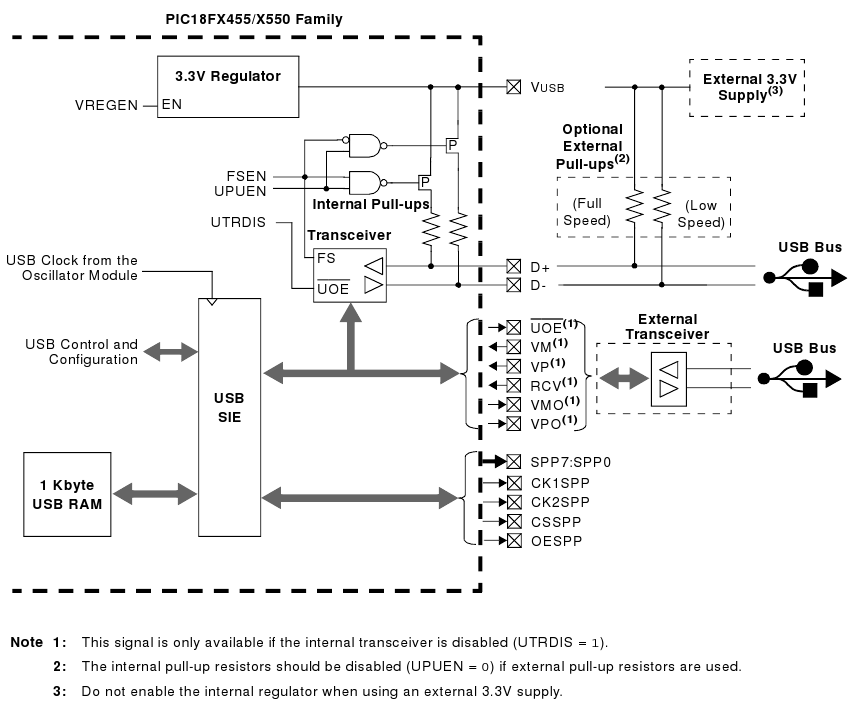
\includegraphics[scale=0.5]{./img/pic_usb_internal.png}
\caption{Arquitectura USB de la familia PIC18FX455/X550.}
\label{fig:pic_usb_internal}
\end{figure}


\subsection{Registros}
El modulo USB es controlado mediante 22 registros disponibles en el
microcontrolador, la mayor\'ia de los cuales son de lectura y escritura.
A continuaci\'on se describir\'an en brevedad cada registro implicado en
\'este trabajo.

\subsubsection{UCON}
% Generar una ref para el apendice del datasheet del 18f4550
El registro \emph{UCON} \footnote{Para m\'as detalles referirse a la hoja de
datos del dispositivo p\'agina 164} posee los bits necesarios para controlar el
modulo USB durante las transferencias. De aqu\'i se controlan:

\begin{itemize}
 \item Activar o desactivar el perif\'erico USB

 \item Reset del puntero del buffer Ping-Pong  

 \item Control del modo \emph{suspend}

 \item Activar o desactivar la transferencia de paquetes
\end{itemize}

\subsubsection{UCFG}
% Generar una ref para el apendice del datasheet del 18f4550
El registro \emph{UCFG} \footnote{Para m\'as detalles referirse a la hoja de
datos del dispositivo p\'agina 165} contiene los bits
necesarios para determinar el comportamiento del modulo USB. Dicho registro
controla:

\begin{itemize}
 \item Velocidad del bus (\emph{Full/Low speed})

 \item Activar o desactivar resistencias internas de Pull-Up

 \item Activar o desactivar el tranceptor interno

 \item Uso del buffer de ping-pong
\end{itemize}

\subsubsection{USTAT}
El registro \emph{USTAT} \footnote{Para m\'as detalles referirse a la hoja de
datos del dispositivo p\'agina 168} contiene la
informaci\'ion espec\'ifica de la \'ultima transferencia recibida. De \'este
registro se puede leer:

\begin{itemize}
 \item Informaci\'on de transacciones en el buffer de ping-pong

 \item N\'umero de enpoint en el que se realiz\'o la \'ultima transacci\'on

 \item Direcci\'on de la ultima transacci\'on (\emph{IN o OUT 'token'})
\end{itemize}

\'Este registro posee un stack del tipo \emph{FIFO} de cuatro niveles que
permite al \emph{SIE} procesar otras transacciones en otros enpoints mientras
el microcontrolador procesa la informaci\'on que se encuentra actualmente en
el registro \emph{USTAT}, como se puede apreciar en la figura
\ref{fig:ustat_fifo}.

% Datasheet pag 168
\begin{figure}[htp]
\centering
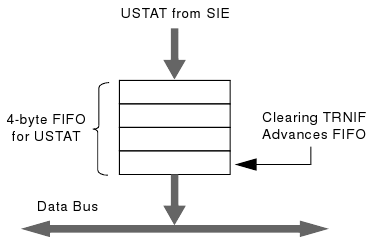
\includegraphics[scale=0.6]{./img/ustat_fifo.png}
\caption{Stack FIFO del registro USTAT.}
\label{fig:ustat_fifo}
\end{figure}

\subsubsection{UEPn}
Los registros \emph{UEPn} \footnote{Para m\'as detalles referirse a la hoja de
datos del dispositivo p\'agina 169} contiene la
configuraci\'on de cada uno de los 16 enpoints. La letra 'n' representa el
n\'umero del enpoint.
Mediante estos registros se puede configurar, para cada endpoint
individualmente, los siguientes par\'ametros:

\begin{itemize}
 \item Activar o desactivar el \emph{handshaking}

 \item Activar o desactivar las transferencias de control (\emph{SETUP})

 \item Activar o desactivar la direcci\'on (\emph{IN o OUT})

 \item Poner el enpoint en modo \emph{STALL}
\end{itemize}


\subsubsection{UADDR}
El registro \emph{UADDR} \footnote{Para m\'as detalles referirse a la hoja de
datos del dispositivo p\'agina 170} contiene la
direcci\'on \'unica que el perif\'erico decodificar\'a una vez activado. Es el
microcontrolador quien debe encargarse de escribir la direcci\'on obtenida
durante el proceso de enumeraci\'on.

%%%%%%%%%%%%%%%%%%%%%%%%%%%%%%%%%%%%%%%%%%%%%%%%%%%%%%%%%%%%%%%%%%%%%%%%%%%%%%
\subsection{USB RAM}
Los datos USB se mueven entre el n\'ucleo del microcontrolador y el \emph{SIE}
mediante un segmento de memoria compartida denominado \emph{USB RAM}.
Este segmento de memoria de puerto dual se encuentra mapeado en espacio de
memoria de datos normal ubicada en el Banco 4 en la direcci\'on 7 (0x400 hasta
0x7FF) por un total de 1Kb como se observa en la figura \ref{fig:usb_mem}.

% Datasheet pag 170
\begin{figure}[htp]
\centering
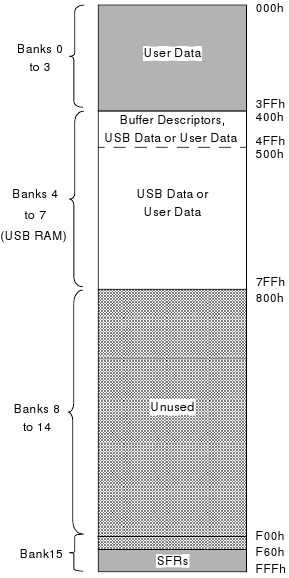
\includegraphics[scale=0.6]{./img/usb_mem.png}
\caption{Mapeo de memoria \emph{USB RAM}.}
\label{fig:usb_mem}
\end{figure}

De \'esta memoria, el Banco 4 (400h a 4FFh), esta dedicada exclusivamente al
control individual de cada endpoint, quedando disponible para uso de datos de
USB la parte no usada del Banco 4 hasta el Banco 7.\\

Por estar mapeada en memoria de datos y siendo accesible tanto por el
microcontrolador como por el \emph{SIE}, la \emph{USB RAM}, se maneja mediante
un sistema de sem\'aforos, asegurando de \'esta manera que un solo dispositivo
este accediendo al mismo segmento de memoria a la vez.

\subsection{Descriptores de Buffer y Tabla de Descriptores de Buffers}
\label{cap:usb_byte}
Para proveerle cierta flexibilidad al usuario, el m\'odulo USB hace uso de
una estructura particular de datos donde se describen los \emph{endpoints} del
USB denominada \emph{Buffer Descriptor Table (BDT)}. \\

La BDT se compone de \emph{Buffer Descriptors (BDs)} los cuales, a su vez, se
componen de 4 registros:

\begin{itemize}
 \item BDnSTAT: Registro de estado del BD

 \item BDnCNT:  Registro de tama\~no de bloque de memoria del BD

 \item BDnADRH: Direcci\'on alta del BD

 \item BDnADRL: Direcci\'on baja del BD
\end{itemize}

\'Esta disposici\'on se puede apreciar mejor en la figura \ref{fig:pic_bdt}.

% Datasheet pag 171
\begin{figure}[htp]
\centering
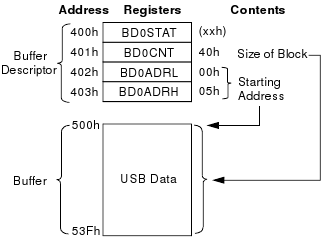
\includegraphics[scale=0.6]{./img/pic_bdt.png}
\caption{Tabla de descriptores de Buffers\emph{BDT}.}
\label{fig:pic_bdt}
\end{figure}

\subsection{BDn}
Los \emph{BDs} se componen de 4 registros (o bytes) por lo que cada
\emph{BDnSTAT} se encuentra siempre siempre a 4n-1 bytes de distancia de la
direcci\'on 400h.\\

\'Este registro tiene la particularidad de poseer un comportamiento que
depende de su contexto.

\subsubsection{Modo CPU}
Cuando \emph{UOWN} = 0 (\emph{BDnSTAT$<7>$}), el microcontrolador posee el
control sobre dicho \emph{BD}. Del registro \emph{BDnSTAT} se destacan los
siguientes bits:

\begin{itemize}
 \item bit 7 - \emph{UOWN}: Se encuentra en 0 cuando el \emph{BD} le pertenece
al microcontrolador

 \item bit 2 - \emph{BSTALL}: Activad o desactivar el estado \emph{STALL}

 \item bit 1-0 - \emph{BC9:BC8}: Los dos bits m\'as significantes del
contador, quien determina el tama\~no del los datos \emph{IN} o \emph{OUT}.
\end{itemize}

El registro \emph{BDnCNT} contiene los bits 7:0 que determinan el tama\~no del
buffer. De esta manera los buffers se limitan a un tama\~no espec\'ifico que
ser\'a el que se puede recibir en una transferencia \emph{OUT}. Mientras que
en una transferencia \emph{IN} se fija el tama\~no del dato que se
transmitir\'a al host.\\

En cuanto a los registros \emph{BDnADRL} y \emph{BDnADRH} poseen la
direcci\'on de USB RAM de los endpoints. El microcontrolador no posee ning\'un
mecanismo intr\'inseco que valide dicha direcc\'ion, lo cual deber\'ia hacerse
mediante software.\\

\subsubsection{Modo SIE}
Cuando \emph{UOWN} = 1 (\emph{BDnSTAT$<7>$}), el \emph{BD} se encuentra bajo
el control del \emph{SIE}. Luego los bits de \'este registro adquieren otro
significado:

\begin{itemize}
 \item bit 7 - \emph{UOWN}: Se encuentra en 1 cuando el \emph{BD} le pertenece
al \emph{SIE}

 \item bit 5-4 - \emph{PID3:0}: Poseen el \emph{PID} de la transacci\'on
(\emph{IN, OUT, SETUP})

 \item bit 1-0 - \emph{BC9:BC8}: Los dos bits m\'as significantes del
contador, quien determina el tama\~no del los datos \emph{IN} o \emph{OUT}.
\end{itemize}

El registro \emph{BDnCNT} contiene los bits 7:0 que determinan el tama\~no del
buffer. Es el \emph{SIE} quien actualiza estos valores seg\'un la ultima
transacci\'on efectuada. En una transacci\'on del tipo \emph{OUT}, el
\emph{SIE} compara el tama\~no del dato recibido si supera el que esta
definido en este registro autom\'aticamente se emite una se\~nal del tipo
\emph{NAK}. Cuando se hace un \emph{IN}, el \emph{SIE} actualiza este registro
con la cantidad de datos enviados.\
Con este m\'etodo es posible luego hacer chequeos del resultado verdadero de
las transacci\'ones USB. 


